\documentclass[11pt]{article}
% common.tex — minimal noise setup
% ----------------------------

% Silence package messages before anything else
\RequirePackage{silence}

% Completely hide "info" messages from LaTeX packages
\WarningFilter*{latex}{}
\WarningFilter*{hyperref}{}
\WarningFilter*{pgf}{}
\WarningFilter*{tikz}{}

% Optionally: hide some hyperref PDF string warnings that are common but harmless
\WarningFilter{hyperref}{Token not allowed in a PDF string}

% ----------------------------
% Now load the usual packages
\usepackage[utf8]{inputenc}
\usepackage[T1]{fontenc}
\usepackage{amsmath, amssymb, amsthm, amsfonts}
\usepackage{geometry}
\usepackage{hyperref}
\usepackage{graphicx}
\usepackage{physics}
\usepackage{booktabs}
\usepackage{listings}
\usepackage{bookmark}
\usepackage{amscd}
\usepackage{tikz-cd}
\usepackage{mathtools}
\usepackage{xspace}
\usepackage[backend=biber, style=numeric]{biblatex}
\usepackage{glossaries}
\usepackage{tcolorbox}

% ----------------------------
% Theorems, macros
\newtheorem{lemma}{Lemma}
\newcommand{\IaMe}{\(IaM^e\)\xspace}
\newcommand{\pdflink}[1]{}

% ----------------------------
% Page layout
\geometry{letterpaper, margin=1in}
\setlength{\parindent}{0pt}
\setlength{\parskip}{1em}

% Hyperref settings
\hypersetup{
    colorlinks=true,
    linkcolor=black,
    citecolor=black,
    filecolor=magenta,
    urlcolor=blue
}

% TOC formatting
\usepackage{tocloft}
\setlength{\cftbeforechapskip}{1.0em}
\setlength{\cftbeforesecskip}{0pt}
\setlength{\cftbeforesubsecskip}{0pt}
\renewcommand{\cftchapleader}{\cftdotfill{\cftdotsep}}

% Glossary
\defglsentryfmt{\ifglsused{\glslabel}{\glsgenentryfmt}{\textit{\glsgenentryfmt}}}

% Author
\author{$IaM^e$}


\input{../glossary.tex}
\addbibresource{../references.bib}

\title{Spectral Minimality and Structure Formation in High-Entropy Wavefunction Ensembles}

\date{\today}

\begin{document}

\maketitle

\begin{abstract}
We extend a minimal information-theoretic model of structure formation from discrete bitstring dynamics to continuous complex-valued wavefunctions defined over spacetime. In the original formulation, increasing entropy in a finite binary sequence led to the emergence of hierarchical structures under simple pattern-detection rules. 

Here, we generalize this idea by defining a variational problem over a spacetime wavefunction $\Psi(x,y,t)$, constrained to follow a prescribed entropy trajectory while minimizing spectral complexity. The resulting optimized configurations exhibit persistent, spatially localized structures even in high-entropy regimes.

This demonstrates that structure can arise not from low entropy alone, but from global constraints on representation complexity. The results suggest that increasing entropy expands the space of accessible configurations, within which structured subregions emerge as stable features under minimal-description principles.
\end{abstract}


\section{Introduction}

In earlier work, we introduced a minimal computational model in which a finite bitstring evolves from a zero-entropy state through random mutations. As entropy increases, simple pattern-detection rules applied to the bitstring reveal the emergence of hierarchical structures. This demonstrated that increasing entropy does not preclude structure, but rather enables the formation of statistically stable patterns within a growing configuration space.

However, the bitstring model is inherently discrete and representation-dependent. A natural question is whether this phenomenon persists in more general settings, particularly in continuous or wave-like representations more closely aligned with physical theories.

In this work, we extend the model to complex-valued wavefunctions defined over a discrete spacetime lattice. Instead of simulating stochastic evolution, we construct spacetime configurations via global variational optimization. The system is constrained to follow a prescribed entropy trajectory while minimizing a spectral complexity functional.

This formulation removes explicit particle definitions and replaces them with a general principle: structures correspond to regions that remain stable under global constraints on representation complexity. We investigate whether such structures arise naturally even in high-entropy regimes.


\section{Model Definition}

\subsection{Wavefunction Representation}

We consider a complex-valued wavefunction:
\[
\Psi : \mathbb{Z}_W \times \mathbb{Z}_H \times \{0, \dots, T-1\} \to \mathbb{C}
\]

For each time slice $t$, we define its Fourier transform:
\[
\Psi_k(t) = \mathcal{F}[\Psi(x,y,t)]
\]

\subsection{Spectral Complexity}

We define spectral complexity as:
\[
C(t) = \sum_k k^2 |\Psi_k(t)|^2
\]

where $k^2 = k_x^2 + k_y^2$ denotes squared frequency magnitude.

\subsection{Probability and Entropy}

To obtain a stable and controllable entropy profile, we define the spatial probability distribution using a temperature-scaled transformation of the amplitude:

\[
p(x,y,t) = \frac{\exp\left(\beta(t) \log(|\Psi(x,y,t)|^2 + \epsilon)\right)}{\sum_{x,y} \exp\left(\beta(t) \log(|\Psi(x,y,t)|^2 + \epsilon)\right)}
\]

where $\beta(t) > 0$ is a time-dependent inverse temperature parameter, and $\epsilon$ ensures numerical stability.

The Shannon entropy is then:
\[
H(t) = -\sum_{x,y} p(x,y,t)\log p(x,y,t)
\]

This formulation allows direct control over the entropy of each time slice by modulating $\beta(t)$.


\subsection{Target Entropy Schedule}

We impose a smooth entropy trajectory of the form:
\[
H_{\text{target}}(t) = H_{\text{start}} + (H_{\text{end}} - H_{\text{start}})\left(1 - e^{-\kappa \frac{t}{T-1}}\right)
\]

where:
\[
H_{\text{start}} = \alpha_{\text{start}} \log(W \cdot H), \quad
H_{\text{end}} = \alpha_{\text{end}} \log(W \cdot H)
\]

and $\kappa > 0$ controls the rate of approach to the asymptotic entropy.

This formulation allows the system to evolve from intermediate entropy states toward near-maximal entropy.



\section{Numerical Optimization}

We parametrize $\Psi_k(t)$ directly as a learnable tensor in Fourier space and optimize:

\begin{itemize}
    \item Real and imaginary components as independent variables
    \item Gradient descent via Adam optimizer
\end{itemize}

At each iteration:
\begin{enumerate}
    \item Construct $\Psi_k(t)$
    \item Compute inverse FFT to obtain $\Psi(x,y,t)$
    \item Evaluate entropy and complexity
    \item Backpropagate total loss
\end{enumerate}

The optimization is performed globally over all time slices simultaneously.



\section{Results}

The optimized spacetime wavefunction exhibits the following properties:

\subsection{High-Entropy Regime}

For large $t$, entropy approaches its maximum:
\[
H(t) \approx \log(W \cdot H)
\]

The spatial distribution resembles noise, but is not fully random.

\subsection{Localized Structures}

Despite near-maximal entropy, the probability field contains:

\begin{itemize}
    \item spatially localized peaks
    \item coherent interference patterns
\end{itemize}

These structures arise from constructive interference of Fourier modes.

\subsection{Temporal Persistence}

Structures persist across adjacent time slices. This occurs because:

\begin{itemize}
    \item large spectral changes increase $C(t)$
    \item maintaining continuity minimizes total functional cost
\end{itemize}

Thus, the optimizer favors gradual deformation over discontinuous reconfiguration.


\begin{figure}[h!]
\centering
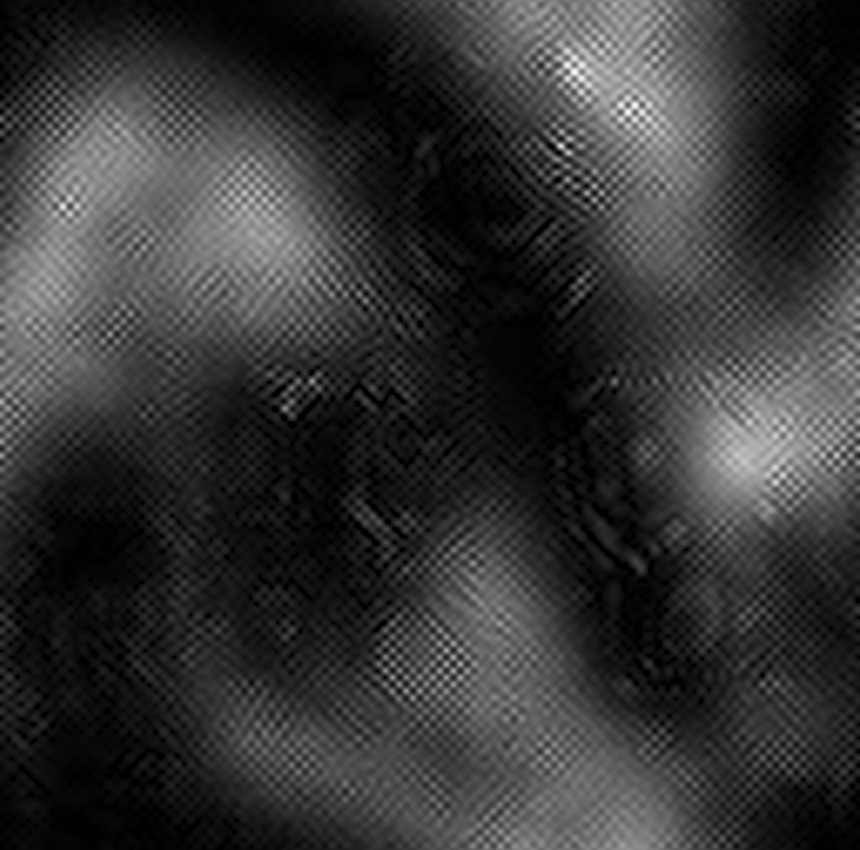
\includegraphics[width=1.0\textwidth]{figures/primordial_soup.png}
\caption{Snapshot of the optimized spacetime wavefunction $|\Psi(x,y,t)|^2$ at a time slice. The field exhibits localized high-probability regions (bright spots) embedded in a high-entropy background. These structures emerge from minimizing the spectral complexity functional under an entropy constraint.}
\end{figure}

\subsection{High-Entropy Regime}

For large $t$, entropy approaches its prescribed upper bound:
\[
H(t) \approx H_{\text{end}}
\]

Despite this, the spatial distribution is not fully uniform. Instead, it exhibits structured deviations from randomness.

\subsection{Localized Structures}

The probability field contains spatially localized peaks and coherent interference patterns. These structures are not imposed explicitly, but arise from the constraint that the wavefunction must simultaneously:

\begin{itemize}
    \item maintain high entropy, and
    \item minimize spectral complexity.
\end{itemize}

This tension leads to configurations in which localized regions concentrate probability mass while the global distribution remains broadly dispersed.

\subsection{Temporal Persistence}

Structures persist across adjacent time slices due to the global nature of the optimization. Large temporal variations would increase spectral complexity, so the optimizer favors configurations that evolve smoothly over time.

This produces coherent trajectories of localized structures, resembling persistent objects in spacetime.



\section{Interpretation}

The results demonstrate that high entropy does not eliminate structure. Instead, increasing entropy expands the space of accessible configurations, within which structured subregions can emerge as stable solutions under global constraints.

In the earlier bitstring model, structure appeared as recurring patterns within an expanding combinatorial space. In the present formulation, structure appears as localized concentrations of probability within a high-entropy field.

In both cases, the underlying mechanism is the same: entropy increase enlarges the configuration space, while constraints on representation (such as spectral minimality) select structured configurations within that space.

This suggests that structure is not in opposition to entropy, but rather a consequence of constrained optimization within high-entropy ensembles.locality constraints, interaction potentials nor predefined object models.


\section{Future Work}

Potential extensions include definition of observer functionals over $\Psi(x,y,t)$



\section{Conclusion}

We have extended a discrete, entropy-driven model of structure formation to a continuous wavefunction-based framework. By imposing a prescribed entropy trajectory and minimizing spectral complexity, we construct spacetime configurations that exhibit persistent, localized structures even near maximal entropy.

These results support the view that structure emerges not from low entropy alone, but from the interplay between entropy and global constraints on representation. Increasing entropy expands the space of possible configurations, while minimal-complexity principles select structured solutions within that space.

This provides a unified perspective in which spacetime structure and matter-like features arise naturally from information-theoretic principles, without requiring explicit physical interaction laws.



\section{Simulation Code}

\begin{itemize}
    \item \href{simulations/block_universe_variational_solver.py}{\texttt{block\_universe\_variational\_solver.py}: Spacetime Variational Wavefunction Solver}
\end{itemize}
   
\printbibliography


\end{document}
